\documentclass[11pt,a4paper]{article}
\usepackage[utf8]{inputenc}
\usepackage[german]{babel}
\usepackage{amsmath}
\usepackage{amsfonts}
\usepackage{amssymb}
\usepackage{graphicx}
\usepackage[left=2cm,right=2cm,top=2cm,bottom=1.8cm]{geometry}

\author{AlphaNerd}
\title{Systeme Wissensfragen}

\begin{document}
\maketitle


\subsection*{Kapitel 2: Überblick}
\begin{itemize}
\item[1)]
Verschiedene Arten von Betriebssystemen werden für verschiedene Verwendungszwecke benutzt. Nennen sie 4 Arten von Betriebssystemen.
\begin{enumerate}
\item Echtzeit-BS
\item Server-BS
\item Embedded-Systems-BS
\item PC-BS
\item Mainframe-BS
\end{enumerate}
\end{itemize}


\subsection*{Kaptiel 3: Dateisytseme}
\begin{itemize}
\item[1)] Nennen sie 5 Dateiattribute (Metadaten) die vom Betriebssystem angelegt werden.

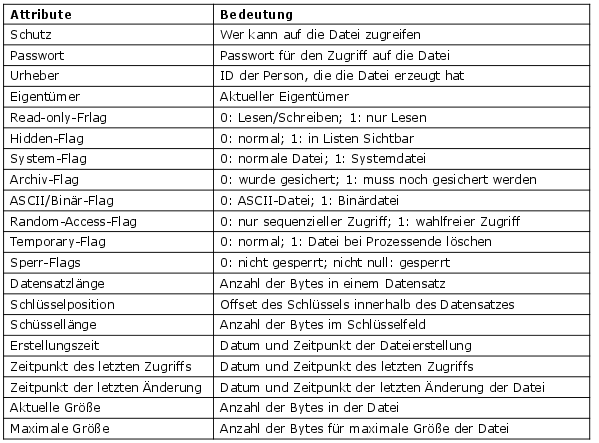
\includegraphics[scale=0.8]{dateiattribute.png}

\item[2)] Wie unterscheiden sich die rwx Rechte für Dateien und Verzeichnisse?

\textbf{Read} gleich. \textbf{Write} bei Verzeichnissen: neue Objekte anlegen. \textbf{Execute} bei Verzeichnissen: Betreten und Objekte ausführen. (Anmerkung: Es ist kein execute recht nötig um Objekte anzulegen in Verzeichnissen! D.h. ohne in das Verzeichnis wechseln zu dürfen, können Objekte angelegt werden.)

\item[3)] Welche Auswirkung hat das setzen des SUID- bzw. SGID-Flags auf die Dateirechteverteilung?

SUID: Ausführung (für alle User) mit Rechten des Besitzers.\\
SGID: Ausführung (für alle USer) mit Rechten der besitzenden Gruppe.

\item[4)] Wie verhalten sich mit \texttt{ln -s QUELLE ZIEL} erstellte Dateien im Vergleich zu mit \texttt{ln QUELLE ZIEL} erstellte Dateien? Sind Verzeichnisse als \texttt{QUELLE} gültig?\\

\texttt{ln -s QUELLE ZIEL}: Symbolischer Link, als Zeiger, unterschiedliche Rechte als Quelle, bei Löschen von Quelle zeigt er ins leere, Partitionsunabhängig, eigene Inode, eigener Name.\\
\texttt{ln QUELLE ZIEL}: Hard Link, eigene Instanz des Dateiobjekts, bei Erstellen gleiche Rechte.\\
\\ Nur bei Softlinks möglich, bei Hardlinks könnte es Kreisschlüsse geben.


\item[5)] Geben sie die minimale Zugriffszeit auf das n-te Byte bei a) Sequentiellen Speichertypen und b) Random-Access-Memory an.
\begin{itemize}
\item[a)] O(n), da über alle vorheriger Bits.
\item[b)] O(1), da konstanter Zugriff. 
\end{itemize}

\item[6)] Geben sie 6 Systemaufrufe (Operationen) auf a) Dateien und b) Verzeichnisse an.
\begin{itemize}
\item[a)] Delete, Create, Read, Write, Open, Close, GetAttribute, SetAttribute, rename, append, seek, ...
\item[b)] Delete, Create, ReadDir, OpenDir, CloseDir, GetAttribute, SetAttribute, rename, ..
\end{itemize}


\item[7)] Welche Vor- und Nachteile besitzt die Realisierung von Dateien als zusammenhängende Belegung (2 Nennungen)? Wo wird diese eingesetzt?
\begin{itemize}
\item[] \textbf{Positiv:} Lesegeschwindigkeit, keine Interne Fragmentierung, kein Speicheroverhead
\item[] \textbf{Negativ:} Dateigröße muss feststehen, hohe externe Fragmentierung, Verwaltungsaufwand durch Defragmentierung.
\item[] \textbf{Verwendung:} Medien die nur einmalig beschrieben werden, z.B. CD, Backup, ..
\end{itemize}

\item[8)] Welche Vor- und Nachteile besitzt die Realisierung von Dateien als verkettete Listen auf der Festplatte (3 Nennungen)? Wie verändern sich diese beim benutzen einer FAT?
\begin{itemize}
\item[] \textbf{Vorteile:} Interne Fragmentierung nur bei letztem Glied, keine externe Fragmentierung, Dateien beliebiger größer anlegbar.
\item[] \textbf{Nachteile:} Langsamer zugriff, (Overhead durch Zeiger)
\item[] \textbf{FAT:} Schnellere Zugriffe, durch Fat im Hauptspeicher. Aber FAT belegt Speicherplatz im Hauptspeicher (unabhängig von aktueller Anzahl an benutzten Dateiblöcken).
\end{itemize}

\item[9)] Welchen Einfluss hat die Wahl der Blockgröße auf die Performance eines Fat32 Dateisystems?\\

Kleinere Blöcke bedeuten weniger interne Fragmentierung, jedoch ist die FAT größer (mehr Zeiger). Größere blöcke komplementär. Maximale Größe des Dateisystems wird durch Blockgröße begrenzt. 


\pagebreak

\item[10)] RAID 0: Striping \\RAID 1: Mirroring \\ RAID 5: Block-Level Striping mit verteilter Parität.
\\\\Skizzieren sie die Realisierung von RAID 0/1/5.\\
\\
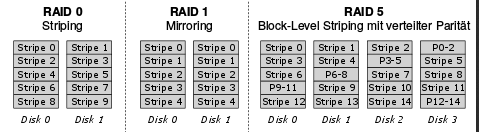
\includegraphics[scale=1]{raid.png}

\end{itemize}


\subsection*{Kapitel 4: Prozesse}
\begin{itemize}
\item[1)] Erklären sie den Unterschied zwischen Programm, Prozess und Threads. Welche Informationen werden jeweils verwaltet (jeweils 3 Nennungen). 

Ein Programm ist ein implementierter Algorithmus, folgende Informationen werden verwaltet:
\begin{enumerate}
\item Programmdaten
\item Programmvorschrift
\item Metadaten
\end{enumerate}
Ein Prozess ist eine Instanz eines Programmes, folgende Informationen werden verwaltet:
\begin{enumerate}
\item Programmcounter (PC)
\item Registerinhalte
\item Variablen Belegung
\end{enumerate}
Ein Thread ist ein Unterprozess mit geteiltem Namensraum, folgende Informationen werden verwaltet:
\begin{enumerate}
\item Programmcounter (PC)*
\item Registerinhalte
\item Variablen Belegung
\end{enumerate}
\item[2)] Wie funktioniert Pseudoparallelität?

Abwechselnde Ausführung von Prozessen mit geringem Quantum.

\item[3)] Zeichnen sie ein Zustandsdiagramm für Prozesse mit Nichtpräemptivem und prämptivem Scheduling, mit und ohne Auslagerung.

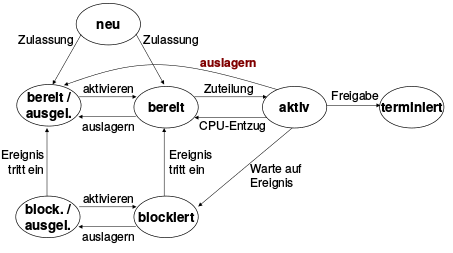
\includegraphics[scale=0.95]{zustand.png}
\end{itemize}


\subsection*{Kapitel 5: Nebenläufigkeit}
\begin{itemize}
\item[1)] Erläutern sie den Begriff \glqq Racecondition\grqq.

Zwei oder mehr Prozesse benutzen die selbe Ressource und das Ergebnis hängt von der Ausführungsreihenfolge ab.
\item[2)] Nennen sie die 4 Anforderungen an Lösungen für das Problem der kritischen Region.
\begin{enumerate}
\item Wechselseitiger Ausschluss
\item Kein Prozess darf ewig warten auf Eintritt in die Kritische Region
\item Keine Annahme über Geschwindigkeit und Anzahl der Prozessorkerne
\item Prozess ausserhalb der kritischen Region dürfen keine anderen Blockieren
\end{enumerate}
\item[3)] Wie wollen die Tutoren umbedingt einen Widerspruchsbeweis strukturiert haben?

Siehe 4.)
\item[4)] Beweisen sie, dass durch diese Implementierung ein wechselseitiger Ausschluss garntiert ist. Welcher Nachteil ergibt sich durch diese Realisierung?\\
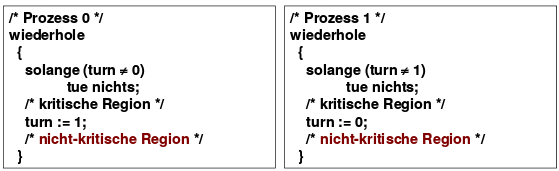
\includegraphics[scale=0.7]{kap5strikt.png}

Beweis:
\begin{itemize}
\item[] \textbf{Behauptung:} Der Wechselseitige Ausschluss ist garantiert.
\item[] \textbf{Beweis:} Durch Widerspruch
\item[] \textbf{Annahme:} o.B.d.A geht P1 zuerst in die kritische Region zum Zeitpunkt $t_1$. P0 geht nach P1 zum Zeitpunkt $t_0$ in die kritische Region ein. Zu $t_1$ ist turn=1. Folglich muss zwischen $t_0$ und $t_1$ muss turn auf 0 gesetzt werden.
\item[] \textbf{Widerspruch:} Turn kann nicht auf 0 gesetzt werden, wärend P1 in der kritischen Region ist.
\item[] \textbf{Schlussfolgerung:} Behauptung wahr.
\end{itemize}

Der Eintritt in die kritische Region ist nur abwechselnd möglich. Prozesse können verhungern.

\item[5)] Nennen sie den Nachteil von reinen Softwarelösungen für die Lösung für das Problem der kritischen Region.

Aktives Warten.
\item[6)] Nennen und erklären sie einen der Assembler Befehle der für eine atomare Ausführung sorgt.

TSL (Test and set Lock) und bei Intel x86: XCHG. Es das Setzen und Lesen der Lockvariable atomar ausgeführt.
\item[7)] Welchen Nachteile birgt eine reine Hardwarelösung?

Aktives Warten.



\pagebreak


\item[8)] Welche Daten (3) und Operationen (2) besitzt ein Mutex?

Daten:
\begin{enumerate}
\item \texttt{ID}
\item \texttt{LOCK}
\item \texttt{queue}
\end{enumerate}

Operationen
\begin{enumerate}
\item \texttt{mutex\_unlock(ID)}
\item \texttt{mutex\_lock(ID)}
\end{enumerate}
\item[9)] Welche Situation beschreibt a) \texttt{$count_s < 0$} \ \ \ b) \texttt{$count_s = 0$} \ \ und \ c)  \texttt{$count_s > 0$} bei einer Semaphore s?

\begin{itemize}
\item[a)] Weitere Weckrufe stehen schon aus, nächster Prozess legt sich auch schlafen
\item[b)] Keine Weckrufe sind bisher gespeichert, nächster Prozess legt sich schlafen
\item[c)] Frei, nächster Prozess darf fortfahren.
\end{itemize}

\item[10)] Implementieren sie eine Lösung für das Produzenten-Konsumenten-Problem für 2 Produzenten, 2 Konsumenten und einer Buffergröße von n, der Buffer sei Anfangs leer. Achten sie auf die Initialisierung ihrer Semaphoren.

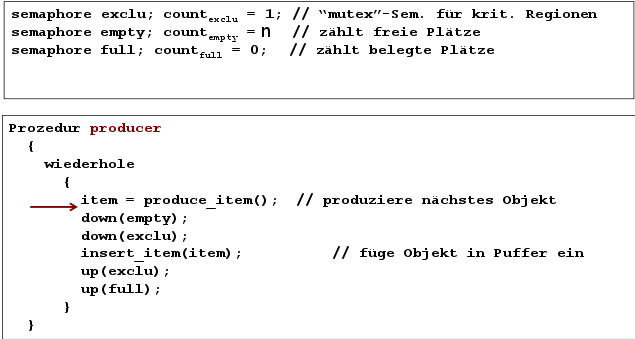
\includegraphics[scale=0.7]{produzent.png}

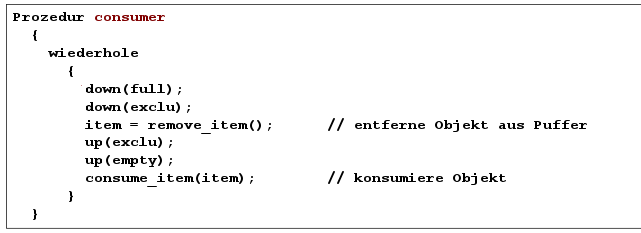
\includegraphics[scale=0.7]{konsument.png}

\end{itemize}


\pagebreak


\subsection*{Kapitel 6: Deadlocks}
\begin{itemize}
\item[1)] Welche 4 Vorraussetzungen müssen für das Auftreten von Deadlocks gegeben sein?

\begin{enumerate}
\item Wechselseitiger Ausschluss
\item Zyklisches Warten: Es gibt eine zyklische Kette von Prozessen, von denen jeder auf eine Ressource wartet, die dem nächsten Prozess in der Kette gehört
\item Besitzen und Warten: Prozesse, die schon Ressourcen reserviert haben, können noch weitere Ressourcen anfordern
\item Kein Ressourcenentzug: Ressourcen, die einem Prozess bewilligt wurden, können nicht gewaltsam wieder entzogen werden
\end{enumerate}


\item[2)] Wann existiert immer eine Ausführungsreihenfolge die zu keinem Deadlock führt?

Genug Ressourcen für sequenzielle Ausführung der Prozesse.

\item[3)] Welche Vorraussetzungen benötigt der Bankieralgorithmus um eine Deadlock freie Ausführungsreihenfolge zu garantieren (2)?

\begin{enumerate}
\item Im Voraus bekannt: Welche und wie viele Ressourcen die einzelnen Prozesse maximal anfordern werden
\item Anforderung übersteigt für keinen Prozess die zur Verfügung stehenden Ressourcen
\end{enumerate}

\item[4)] Warum existiert für manche vom Bankieralgorithmus als unsicher eingestufte Ausführungen trotzdem eine Deadlock freie Restausführung (2 Nennungen)?

Da der Bankieralgorithmus nimmt zwei Dinge an:
\begin{enumerate}
\item Alle Prozesse ihre Anforderungen auf einen Schlag stellen.
\item Die Prozesse erst nach ihrer Terminierung die Ressourcen freigeben. 
\end{enumerate}

\item[5)] Welche Matrizen benötigt der Bankieralgorithmus?

\begin{enumerate}
\item A: Noch angeforderte Ressourcen
\item E: Erhaltene Ressourcen
\item V: Vorhandene Ressourcen
\item M: Maximale Anforderungen
\item F: Freie Ressourcen
\end{enumerate}

\item[6)] Warum ist durch den Bankieralgorithmus das Deadlockproblem nicht restlos gelöst (3 Nennungen)?

\begin{enumerate}
\item Maximalen Anforderungen müssen bekannt sein.
\item Mehr Anforderungen als Ressourcen kann es trotzdem eine deadlockfreie Restausführung geben.
\item Anzahl der Prozesse nicht immer konstant/statisch.
\end{enumerate}

\pagebreak


\item[7)] Welche Bewältigungsstrategien gibt es für die Behebung von Deadlocks (2 Nennungen)?
\begin{enumerate}
\item Abbruch aller verklemmten Prozesse 
\item Rückführung aller verklemmten Prozesse auf einen festgelegten Kontrollpunkt und Neustart
\item Schrittweiser Abbruch aller verklemmten Prozesse, bis die Verklemmung nicht mehr existiert
\item Schrittweiser Ressourcenentzug,  bis die Verklemmung nicht mehr existiert 
\end{enumerate}
\end{itemize}

\subsection*{Kapitel 7: Scheduling}
\begin{itemize}
\item[1)] Nennen und beschreiben sie die 3 Arten von Scheduling.

\begin{enumerate}
\item Langfristiges: Welche Prozesse werden zugelassen.
\item Mittelfristiges: Welche Prozesse werden ausgelagert.
\item Kurzfristiges: Welche Prozesse bekommen CPU zugeteilt.
\end{enumerate}

\item[2)] Worin liegt der Unterschied zwischen Benutzer- und Systemorientiertem Scheduling (3 Nennungen)?

Der Benutzer will eine möglichst geringe durchschnittliche Durchlaufzeit. Systemorientiert bedeutet, es soll ein möglichst hoher Durchsatz erreicht werden.


\item[3)] Bestimmen sie die Auswahlfunktion, sowie die Zuordnung zu nicht- beziehungsweise präemptivem Scheduling von folgenden Strategien:
\begin{enumerate}
\item First Come First Served (FCFS)
\item Round Robin (RR)
\item Shortest Job First (SJF)
\item Shortest Remaining Time (SRT)
\item Highest Response Ratio Next (HRRN)
\end{enumerate}

\begin{enumerate}
\item max(w), nicht prämptiv.
\item max(w) (nach queue), präemptiv, mit Quantum.
\item min(s), nicht präemptiv.
\item min(s-e), präemptiv, jedes mal wenn neuer Prozess bereit ist.
\item max((w+s)/s), nicht präemptiv
\end{enumerate}

\item[4)] Erläutern sie kurz Feedback beziehungsweise Unixscheduling.

Feedback: Mehrere Prioritäten, jeweils mit eigener Warteschleife. Innerhalb einer Priorität FCFS und in letzter RR.


\pagebreak


\item[5)] Analysieren sie die Schedulingstrategien aus Aufgabe 3 in Hinsicht auf a) Bevorzugung von kurzen/langen Prozessen, b) Livelock Gefahr, c) eventuellen Wissensanforderungen und d) Effektivität im Sinne der Benutzer- beziehungsweise Systemorientierter Anwendung.\\

\begin{tabular}{|p{1.2cm} ||p{3cm}|p{3cm}|p{3cm}|p{3.6cm}|}
\hline 
 & a) Bevorzugung & b) Livelockgefahr & c) Wissensanforderung & d) Benutzer/System\\ 
\hline
\hline 
FCFS & Bevorzugt lange & Nein & Nein & Für beide nicht interessant \\ 
\hline 
RR & Bevorzugt Prozesse ohne E/A & Nein & Nein & Nicht sehr interessant \\ 
\hline 
SJF & Bevorzugt kurze Prozesse & Ja, für lange Prozesse & Die Gesamtlaufzeit muss bekannt sein & Gut für Benutzer \\ 
\hline 
SRT & Bevorzugt kurze & Ja, für lange Prozesse & Die Gesamtlaufzeit muss bekannt sein & Beste für Benutzer \\ 
\hline 
HRRN & Bevorzugt kurze & Nein & Ja, Gesamtlaufzeit muss bekannt sein & Ausgeglichen \\ 
\hline 
\end{tabular} 
\end{itemize}
o

\subsection*{Kapitel 8: Speicherverwaltung}
\begin{itemize}
\item[1)] Skizzieren sie die Speicherhierache (5 Nennungen).

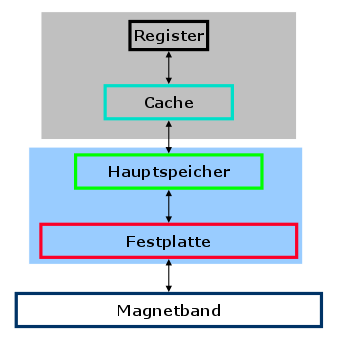
\includegraphics[scale=0.6]{hierachie.png}

\item[2)] Welche 5 Anforderungen werden an die Speicherverwaltung gestellt? Erläutern sie diese kurz.

\begin{enumerate}
\item \textbf{Relokation:} Auslagern und Einlagern von Prozessen aus dem Hauptspeicher muss möglich sein.
\item \textbf{Schutz:} Namensräume von Prozessen müssen vor Zugriffen durch andere Prozesse gesichert sein.
\item \textbf{Gemeinsame Nutzung:} Prozesse können über ein Shared-Memory kollaborieren.
\item \textbf{Physische Organisation:} Implementierung des Speichers.
\item \textbf{Logische Organisation:} Modularität möglich.
\end{enumerate}

\item[3)] Wie stehen physikalische, logische und relative Adressen im Zusammenhang?

Die physikalische ist reale Addresse im Speicher und die logische ist diejenige, die innerhalb eines Programmes verwendet wird. Die relative ist ein Spezialfall der logischen Adresse, es wird bezug auf (z.B) Programmanfang genommen.

\item[4)] Wie können Namensräume von Prozessen vor einander geschützt werden? Skizzieren sie.

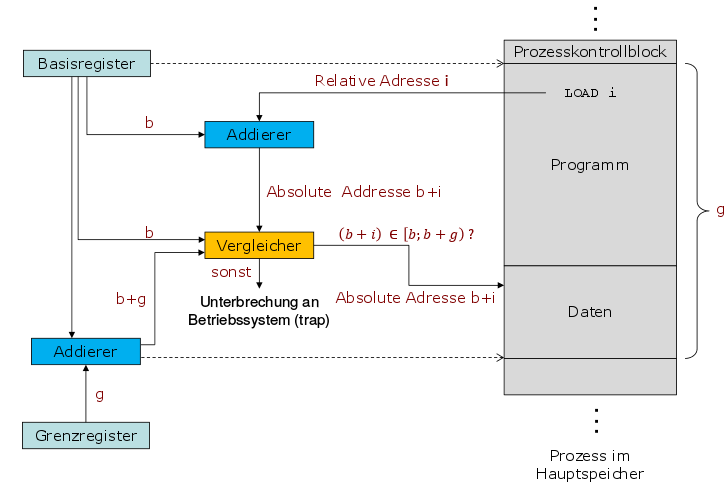
\includegraphics[scale=0.6]{schutz.png}

\item[5)] Welche Vor- und Nachteile treten bei den drei Varianten der Partitionierung auf? (Jeweils 3, 3 und 1 Nennungen.

\begin{enumerate}
\item Statische Partitionierung (feste und variable Größe)
\begin{itemize}
\item Vorteile: Keine externe Fragmentierung, Geringer Verwaltungsaufwand.
\item Nachteile: Begrenzte Anzahl und Größe von Prozessen, hohe Interne Fragmentierung.
\end{itemize}

\item Dynamische Partitionierung
\begin{itemize}
\item Vorteile: Keine interne Fragmentierung, Prozesse variabler länge.
\item Nachteile: Hohe externe Fragmentierung nach Ein-/Auslagerung und hoher Verwaltungsaufwand.
\end{itemize}

\item Buddy System
\begin{itemize}
\item Vorteile: Weniger als halbe Blockgröße interne Fragmentierung. Externe Fragmentierung löst sich selbstständig auf. Geringer Verwaltungsaufwand.
\item Nachteile: 
\end{itemize}

\end{enumerate}

\item[6)] Nennen sie die drei Speicherzuteilungsalgorithmen, welcher ist am effektivsten? Welche Nebeneffekte treten bei den anderen beiden auf?

\begin{enumerate}
\item Next Fit: Etwas schlechter als First Fit, typischer Effekt: Fragmentierung am Ende des Speichers.
\item First Fit: Ist beste.
\item Best Fit: Suche braucht Zeit. Hohe Fragmentierung durch viele kleine Partitionen.
\end{enumerate}

\item[7)] Welche Größe muss das Offset-Feld beim einfachen Paging mindestens haben, wenn die Seitengröße $2^{11}$ Bit beträgt (Zeilengröße $2^4$ Bit)?



\item[8)] Erklären sie den Begriff des virtuellen Speichers. Welche Vor- und Nachteile ergeben sich dadurch (jew. 2 Nennungen)? Durch welches Prinzip ist die Verwendung trotzdem sinnvoll? Was würde ohne dieses Prinzip passieren?

Virtueller Speicher ist die Einheit aus Hauptspeicher und Swapping Area.

\begin{itemize}
\item Vorteil: Mehr Speicher, größerer Namensraum, Größe von Prozessen müssen nicht im vorraus bekannt sein.
\item Nachteile: Höherer Verwaltungsaufwand durch Ein-/Auslagerung,  
\end{itemize}

Sinnvoll durch das Prinzip der Lokalität, da sonst zuviel Thrashing stattfinden würde.
 

\pagebreak
 
 
\item[9)] Welche Einträge besitzt die Seitentabelle bei Paging mit virtuellem Speicher?

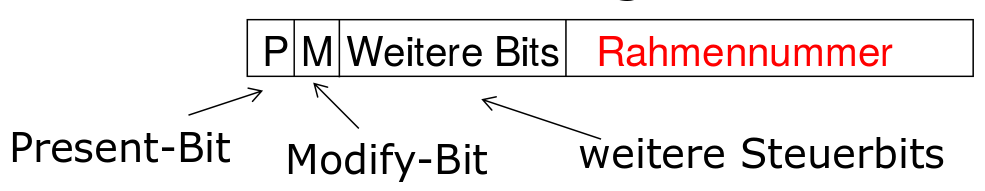
\includegraphics[scale=0.5]{seitentabelle.png}

\item[10)] Skizzieren sie die Adressumsetzung für Paging mit virtuellem Speicher.

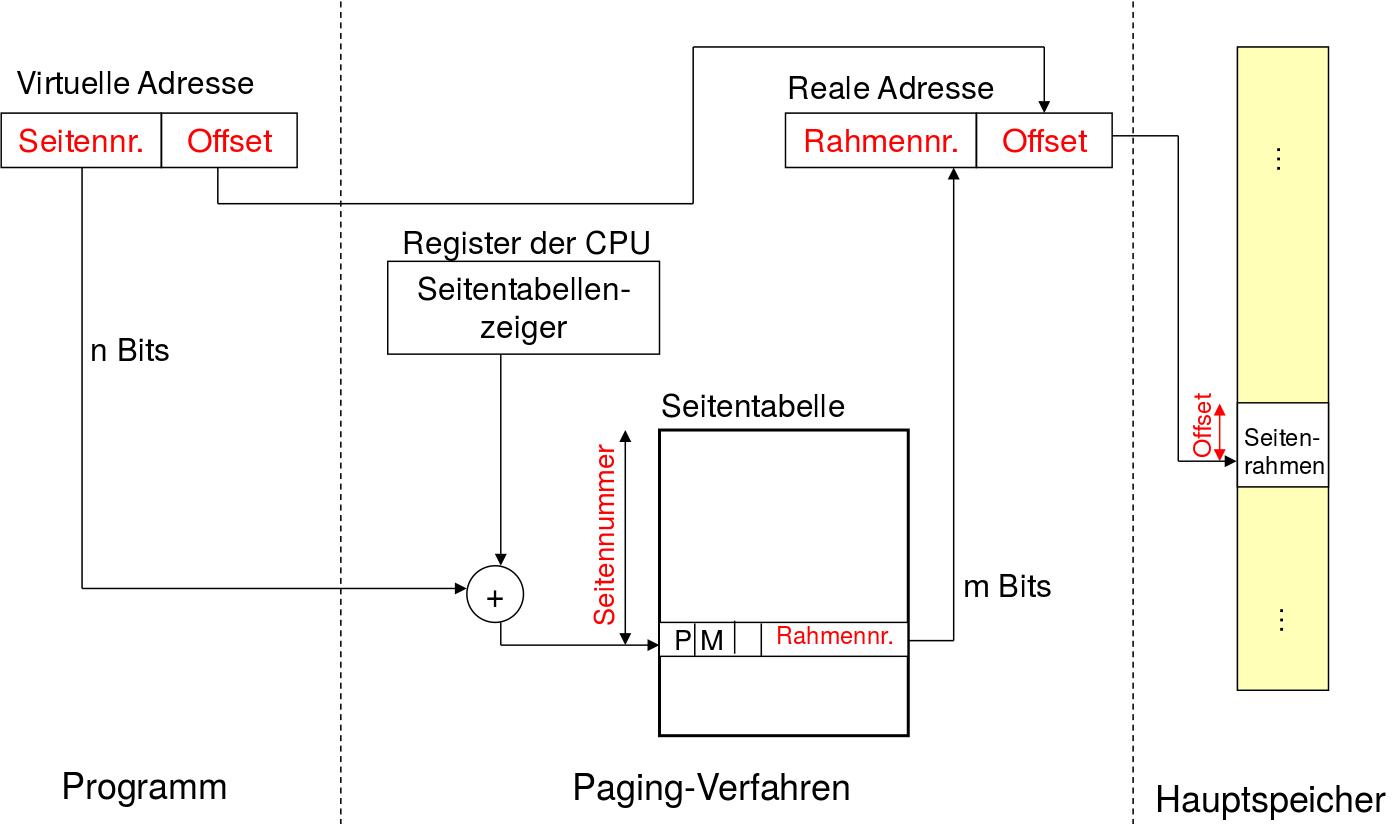
\includegraphics[scale=0.5]{adress.png}

\item[11)] Beschreiben sie kurz das Prinzip der mehrstufigen Seitentabellen.

Zuerst wird die Hauptseitentabelle adressiert und von dort die Addresse der richigen Untertabelle entnommen. Dann analog zum einfachen Paging. 

\item[12)] Beschreiben sie kurz das Prinzip der invertierten Seitentabellen, gehen sie dabei auch auf die Adressumsetzung ein.

Für eine gegebene Seitennummer wird über eine Hash-Funktionen die Stelle in der Seitentabelle berechnet, an der die entsprechende Rahmennummer steht. Sofern hier die Rahmennummer einer anderen Seite steht, wird die Überläuferkette verfolgt, bis Rahmennummer zur gegebenen Seitennummer ausgegeben werden kann.

\item[13)] Beschreiben sie die Grundidee der Speicherverwaltung durch Segmentierung.

Dynamisch wachsend und schrumpfende Speicherabschnitte bilden Segmente. Adressumsetzung ist ähnlich dem des Paging.

\item[14)] Nennen sie 2 Austauschstrategien.
\begin{enumerate}
\item \textbf{F}irst \textbf{I}n \textbf{F}irst \textbf{O}ut (FIFO)
\item \textbf{L}east \textbf{R}ecently \textbf{U}sed (LRU)
\item Clock-Algorithmus
\end{enumerate}
\end{itemize}


\pagebreak


\subsection*{Kapitel 9: Sicherheit}
\begin{itemize}
\item[1)] Worin besteht der Unterschied zwischen Betriebs- und Angriffssicherheit?

Die Betriebssicherheit bezieht sich auf Aspekte, die ohne das Zutun äußerer Einflüsse entstehen können.
Die Angriffssicherheit bezieht sich nur auf eben diese.

\item[2)] Nennen sie die 4 Sicherheitsziele.

\begin{enumerate}
\item Privacy
\item Datenintegrität
\item Systemverfügbarkeit
\item Vertraulichkeit der Daten (data confidientiality)
\end{enumerate}

\item[3)] Nennen sie 2 Verschlüsselungsstrategien.

\begin{enumerate}
\item Symmetrisch Verschlüsselungsstrategien (Caesar-Cypher)
\item Asymmetrisch Verschlüsselungsstrategien (RSA)
\end{enumerate}

\end{itemize}











\end{document}